\documentclass[12pt]{article}

\usepackage{times}
\usepackage{graphicx}
\usepackage{amsmath}
\usepackage{geometry}
\usepackage{svg}
\usepackage{hyperref}
\usepackage{cleveref}
\usepackage{cite}
\geometry{a4paper, margin=1in}

\begin{document}

\begin{titlepage}
    \centering
    \vspace*{1in}
    
    {\Huge \textbf{Non-linear Optics Simulations in Attosecond Lasers Using Python}}\\[2cm]
    
    \textit{A Paper Submitted in Partial Fulfillment of the Requirements for the Course}\\[0.5cm]
    
    \textbf{Photonics and Applications}\\[2cm]
    
    \textbf{Author:}\\
    [0.5cm]
    \textbf{John Andrew Kypriotakis}\\[1.5cm]
    
    \textbf{Instructor:}\\
    [0.5cm]
    \textbf{Konstantinos Makris}\\[1.5cm]
    
    \textbf{Institution:}\\
    [0.5cm]
    \textbf{University of Crete}\\
    \textbf{School of Science and Engineering}\\
    \textbf{Department of Physics}\\[2cm]
    
    \textbf{Date:}\\
    [0.5cm]
    \textbf{\today}
    
    \vfill
\end{titlepage}

\newpage

\tableofcontents
\newpage

\section{Introduction}\label{sec:intro}

Non-linear optics (NLO) has emerged as a crucial field in modern photonics, enabling a broad range of applications including frequency conversion, ultrafast spectroscopy, and the generation of attosecond pulses. With the advancement of laser technology, particularly the development of attosecond lasers, it has become possible to probe and manipulate physical processes on the timescale of electron dynamics, which occur on the order of attoseconds (1 as = $10^{-18}$ s).

Attosecond laser pulses, which are some of the shortest bursts of light ever produced, allow scientists to explore the fast-paced world of atomic and molecular dynamics. The study of non-linear interactions in such short timescales opens up new avenues for research and technological development, making the simulation of these processes a subject of significant interest.

This paper aims to explore the simulation of non-linear optical phenomena in attosecond lasers using Python. By leveraging Python's computational libraries and tools, we can model and analyze complex non-linear processes such as:
\begin{itemize}
    \item Comparison of Attosecond and CW Lasers: By comparing the interaction of attosecond laser pulses with CW lasers, the differences in their influence on non-linear optical processes are elucidated, highlighting the unique advantages of ultra-short pulse durations in driving specific non-linear effects.

    \item Kerr Effect: The Kerr phenomenon, a non-linear optical effect where the refractive index of a material changes in response to the intensity of light, is simulated to understand how intense laser fields modify the optical properties of materials, particularly under the influence of attosecond pulses.
    
    \item Quantum Noise Reduction: Quantum noise, a limiting factor in precision measurements and quantum communication, is examined in the context of non-linear interactions. Simulations explore how non-linear processes, particularly in attosecond regimes, can lead to noise reduction, enhancing the signal-to-noise ratio in quantum systems.
    
    \item High-Order Harmonic Generation (HHG): A critical process for generating high-energy photons from lower-energy inputs, HHG is simulated to study how attosecond pulses can drive efficient harmonic generation, a key mechanism for producing extreme ultraviolet (XUV) and soft X-ray radiation.
    
    \item Cross-Phase Modulation (XPM): The interaction of multiple light waves within a non-linear medium, leading to phase changes, is explored through XPM simulations. The effects of attosecond pulses on cross-phase modulation provide insights into advanced signal processing techniques in photonics.
    
    \item Soliton Interactions: Solitons, self-reinforcing solitary waves, are simulated to observe their behavior in non-linear media under attosecond laser excitation. The interactions between solitons, particularly in the context of ultra-fast pulses, reveal new dynamics that are essential for the development of optical communication systems and other photonic applications.
\end{itemize}

Through these simulations, this paper aims to provide a comprehensive understanding of the non-linear optical phenomena that arise when attosecond lasers interact with various media. The results offer valuable insights into the potential applications of attosecond pulses in photonics, as well as the fundamental physics underlying these ultra-fast processes.

This paper is organized as follows: Section \ref{sec:concepts} reviews the fundamental concepts of non-linear optics relevant to attosecond laser interactions. Section \ref{sec:simulation} discusses the Python-based simulation methods used in this study, including the numerical techniques and algorithms implemented. Section \ref{sec:results} presents the results of the simulations, followed by a discussion of the implications of these findings. Finally, Section \ref{sec:conclusion} concludes the paper and suggests possible directions for future research.

\newpage

\section{Fundamental Concepts of Non-linear Optics and Attosecond Lasers}\label{sec:concepts}

Non-linear optics (NLO) is a branch of optics that studies the behavior of light in non-linear media, where the polarization response of the material to the electric field is non-linear. This non-linearity arises primarily at high light intensities, where the electric field of the light induces a non-linear polarization in the medium, leading to a variety of phenomena that do not occur in linear optics. In this section, we review the fundamental concepts and phenomena relevant to the simulations conducted in this study.

\subsection{Attosecond and Continuous Wave (CW) Lasers}

Attosecond lasers, producing pulses with durations on the order of attoseconds ($10^{-18}$ s), allow for the observation and control of electron dynamics within atoms and molecules. These ultra-short pulses are pivotal in studying non-linear optical phenomena at extreme temporal resolutions. In contrast, continuous wave (CW) lasers emit light continuously over time, offering a steady-state field ideal for examining time-independent non-linear effects. The comparison of these two laser types in non-linear interactions reveals insights into the temporal aspects of light-matter interaction and the advantages of attosecond pulses for certain applications.

\subsection{The Kerr Effect}

The Kerr effect, or the optical Kerr effect, refers to the phenomenon where the refractive index of a material changes as a function of the intensity of the light passing through it. Mathematically, this can be described by the equation:
\begin{equation}
n(I) = n_0 + n_2 I,
\end{equation}
where \( n(I) \) is the intensity-dependent refractive index, \( n_0 \) is the linear refractive index, \( n_2 \) is the non-linear refractive index coefficient, and \( I \) is the intensity of the light. The Kerr effect is fundamental to various non-linear optical processes, including self-phase modulation and the formation of solitons.

\subsection{Quantum Noise Reduction}

Quantum noise, inherent to all quantum systems, arises from the uncertainty principle and is a significant factor in limiting the precision of measurements in quantum optics. Non-linear optical processes can lead to noise reduction through mechanisms such as squeezing, where the quantum uncertainty is redistributed between different components of the light field. This paper investigates how non-linear interactions, particularly in the attosecond regime, can reduce quantum noise, thereby enhancing the performance of quantum optical systems.

\subsection{High-Order Harmonic Generation (HHG)}

High-order harmonic generation (HHG) is a non-linear process in which a strong laser field drives the emission of photons at multiples of the fundamental frequency. This process is highly efficient in the attosecond regime, where intense laser pulses interact with gases or solids to produce high harmonics. The physics of HHG is deeply connected with the dynamics of electrons in atoms, making it a crucial tool for generating attosecond pulses and studying ultra-fast phenomena.

\subsection{Cross-Phase Modulation (XPM)}

Cross-phase modulation (XPM) occurs when the phase of a light wave is modulated by the intensity of another co-propagating light wave in a non-linear medium. This phenomenon is closely related to the Kerr effect and is described by the non-linear Schrödinger equation (NLSE). XPM is essential for understanding the interaction between different light fields within a medium, which has applications in wavelength conversion and signal processing in optical communication systems.

\subsection{Soliton Interactions}

Solitons are stable, localized wave packets that maintain their shape while propagating through a non-linear medium. The formation and interaction of solitons are governed by the balance between non-linearity and dispersion in the medium. Soliton interactions, particularly in the context of attosecond pulses, reveal complex dynamics that are of great interest for optical communication, where solitons can be used to transmit information over long distances with minimal distortion.

\newpage

\section{Python-Based Simulation Methods}\label{sec:simulation}

In this section, we detail the Python-based methods and tools employed to simulate the non-linear optical phenomena discussed in this study. Python, with its extensive libraries and community support, provides a powerful platform for performing complex simulations in photonics and non-linear optics. The following subsections outline the computational approaches, algorithms, and specific libraries used to model each of the phenomena investigated.

\subsection{Computational Framework}

The simulations were carried out using Python 3, leveraging several key libraries that are well-suited for numerical computation, data visualization, and scientific research:

\begin{itemize}
    \item \textbf{NumPy}: Used for numerical operations, such as handling arrays, performing mathematical functions, and implementing fast Fourier transforms (FFT).
    \item \textbf{SciPy}: Provides advanced scientific computing functions, including algorithms for solving differential equations and performing integration.
    \item \textbf{Matplotlib and Seaborn}: Utilized for visualizing simulation results, including plotting time-domain and frequency-domain data.
    \item \textbf{QuTiP (Quantum Toolbox in Python)}: Specifically used for quantum optics simulations, including modeling quantum noise and non-linear quantum effects.
    \item \textbf{PyNLO (Python Non-linear Optics Toolkit)}: Employed for simulating specific non-linear optical processes, such as high-order harmonic generation and soliton dynamics.
\end{itemize}

\subsection{Simulation of Attosecond and CW Lasers}

The comparison between attosecond and continuous wave (CW) lasers was modeled by generating synthetic pulse profiles and analyzing their interaction with non-linear media. The following steps were used:

\begin{enumerate}
    \item \textbf{Pulse Generation}: Gaussian pulses were synthesized for attosecond lasers using NumPy, with pulse durations ranging from a few hundred attoseconds to several femtoseconds. CW laser fields were modeled as continuous sinusoidal waves.
    \item \textbf{Interaction with Media}: The electric fields of these pulses were propagated through simulated non-linear media using the split-step Fourier method (SSFM) implemented in SciPy.
    \item \textbf{Analysis}: The output fields were analyzed in both time and frequency domains to assess the impact of pulse duration on non-linear phenomena.
\end{enumerate}

\subsection{Modeling the Kerr Effect}

The Kerr effect was simulated by solving the non-linear Schrödinger equation (NLSE), which governs the propagation of light in a non-linear medium. The key steps involved:

\begin{enumerate}
    \item \textbf{Setting up the NLSE}: The NLSE was discretized using a finite-difference method, allowing for the inclusion of non-linear terms corresponding to the Kerr effect.
    \item \textbf{Numerical Integration}: The equation was solved using a Runge-Kutta method from SciPy's `odeint` function, ensuring stability and accuracy in the presence of high-intensity fields.
    \item \textbf{Visualization}: The refractive index modulation as a function of input intensity was visualized using Matplotlib, showing the non-linear change in phase and its impact on pulse propagation.
\end{enumerate}

\subsection{Quantum Noise Reduction Simulations}

Quantum noise reduction was studied using QuTiP, which provides tools for simulating quantum systems. The steps include:

\begin{enumerate}
    \item \textbf{System Setup}: The quantum system was defined using density matrices and operators representing the non-linear interaction between light and the medium.
    \item \textbf{Simulation of Squeezing}: Non-linear interactions were modeled to observe squeezing effects, where the uncertainty in one quadrature of the field is reduced at the expense of increased uncertainty in the orthogonal quadrature.
    \item \textbf{Noise Analysis}: The resulting quantum noise reduction was quantified by calculating the squeezing parameter and visualizing the noise distribution using Wigner functions.
\end{enumerate}

\subsection{High-Order Harmonic Generation (HHG)}

HHG was simulated using the PyNLO toolkit, which is specifically designed for non-linear optics simulations:

\begin{enumerate}
    \item \textbf{Laser Field Simulation}: An intense laser field was modeled using PyNLO's pulse class, with parameters corresponding to attosecond pulse characteristics.
    \item \textbf{Propagation through a Gas Medium}: The propagation of the pulse through a gas medium, such as argon, was simulated, taking into account non-linear polarization and ionization effects.
    \item \textbf{Harmonic Generation Analysis}: The harmonic spectrum was calculated using Fourier transforms, and the efficiency of harmonic generation was analyzed as a function of pulse intensity and duration.
\end{enumerate}

\subsection{Cross-Phase Modulation (XPM) Simulation}

Cross-phase modulation was modeled by simulating the interaction between two co-propagating laser pulses in a non-linear medium:

\begin{enumerate}
    \item \textbf{Coupled Wave Equations}: The coupled non-linear Schrödinger equations (NLSE) for the two pulses were set up, with cross-phase modulation terms included.
    \item \textbf{Numerical Solution}: The equations were solved using the split-step Fourier method, which allows for efficient handling of both linear and non-linear effects.
    \item \textbf{Phase Shift Visualization}: The phase shift induced by one pulse on the other was calculated and visualized, showing the impact of XPM on the pulse profile and spectrum.
\end{enumerate}

\subsection{Soliton Interaction Simulation}

The interaction of solitons was simulated using the following approach:

\begin{enumerate}
    \item \textbf{Soliton Generation}: Soliton solutions were generated using PyNLO's soliton solver, which provides analytical solutions for solitons in non-linear media.
    \item \textbf{Propagation and Interaction}: Multiple solitons were propagated through the non-linear medium, and their interactions were simulated using the split-step Fourier method.
    \item \textbf{Interaction Dynamics}: The dynamics of soliton interactions, such as fusion, repulsion, and shape preservation, were visualized to understand the complex behavior of solitons under different initial conditions.
\end{enumerate}

\newpage

\section{Results}\label{sec:results}

In this section, we present the results obtained from the simulations of various non-linear optical phenomena using attosecond lasers, as well as continuous wave (CW) lasers for comparison. The results provide insights into the behavior of light in non-linear media, with a focus on the specific phenomena investigated in this study.

\subsection{Comparison of Attosecond and CW Lasers}

The comparison between attosecond and CW lasers revealed significant differences in their interaction with non-linear media. The key findings include:

\begin{itemize}
    \item \textbf{Intensity Distribution}: Attosecond pulses, due to their ultra-short duration, exhibit peak intensities several orders of magnitude higher than CW lasers. This leads to stronger non-linear effects in a shorter interaction length.
    \item \textbf{Spectral Broadening}: Attosecond pulses induce significant spectral broadening, a result of self-phase modulation, which is not observed in CW lasers.
    \item \textbf{Non-linear Response}: The non-linear response of the medium to attosecond pulses is more pronounced, leading to phenomena such as higher-order harmonic generation and soliton formation, which are less prominent with CW lasers (will be discussed in later sections).
\end{itemize}

Figure \ref{fig:atto_vs_cw_waist} illustrates the beam waist for an attosecond pulsed laser vs a CW laser. We can see that the attosecond laser has a much smaller beam waist, which results in a higher peak intensity.

\begin{figure}[!ht]
    \centering
    \includesvg[width=0.8\textwidth]{../images/attovscw.svg}
    \caption{Beam-waist comparison of attosecond and CW lasers after interaction with a non-linear medium.}
    \label{fig:atto_vs_cw_waist}
\end{figure}

Figure \ref{fig:atto_spectrum} shows the spectral broadening of the attosecond laser after interaction with a non-linear medium, highlighting the impact of ultra-short pulse durations on the spectral characteristics of the light.

\begin{figure}[!ht]
    \centering
    \includesvg[width=0.8\textwidth]{../images/attosecond_spectrum.svg}
    \caption{Spectral broadening of attosecond laser after interaction with a non-linear medium.}
    \label{fig:atto_spectrum}
\end{figure}

\subsection{Kerr Effect Simulation}

The simulation of the Kerr effect demonstrated the intensity-dependent change in the refractive index of the medium. The results are summarized as follows:

\begin{itemize}
    \item \textbf{Refractive Index Modulation}: The refractive index increased non-linearly with the intensity of the input light, consistent with the Kerr effect.
    \item \textbf{Beam Profile}: The beam profile exhibited self-focusing behavior due to the intensity-dependent refractive index, leading to changes in the beam's spatial distribution. This effect is more pronounced for attosecond pulses due to their high peak intensities. 
\end{itemize}

Figure \ref{fig:kerr_index} illustrates the intensity-dependent refractive index change due to the Kerr effect. It is clearly visible, indicating the non-linear response of the medium to the intense laser field. For comparison the beam profile evolution under the influence of the Kerr effect is also shown.

\begin{figure}[!ht]
    \centering
    \includesvg[width=0.8\textwidth]{../images/kerr_index.svg}
    \caption{Intensity-dependent refractive index change due to the Kerr effect. Beam profile evolution under the influence of the Kerr effect is also shown for reference.}
    \label{fig:kerr_index}
\end{figure}

Figure \ref{fig:kerr_beam} shows the beam profile evolution under the influence of the Kerr effect. It is clearly visible that the self-focusing behavior of the beam due to the intensity-dependent refractive index affects the beam profile. Both temporal and spatial profiles are affected by the Kerr effect, leading to changes in the beam's characteristics.

\begin{figure}[!ht]
    \centering
    \includesvg[width=0.8\textwidth]{../images/kerr_profiles.svg}
    \caption{Beam profile evolution under the influence of the Kerr effect. Temporal and spatial profiles are presented.}
    \label{fig:kerr_beam}
\end{figure}

\subsection{Quantum Noise Reduction}

The simulation of quantum noise reduction showed that non-linear interactions could effectively reduce quantum noise through squeezing. Figure \ref{fig:quantum_noise} illustrates the comparison of quantum noise in a squeezed state vs an unsqueezed state. The squeezed state exhibits reduced quantum noise, indicating the redistribution of uncertainty between different quadratures of the light field.

\begin{figure}[!ht]
    \centering
    \includesvg[width=0.8\textwidth]{../images/quantum_noise.svg}
    \caption{Comparison of the quantum noise in a squeezed state vs an unsqueezed state. The squeezed state is clearly in reduced quantum noise.}
    \label{fig:quantum_noise}
\end{figure}

\subsection{Optical Soliton Propagation}

The propagation simulation of optical solitons was performed to observe the behavior of these stable, localized wave packets in a non-linear medium. The key findings from the simulation are as follows:

\begin{itemize}
    \item \textbf{Soliton Shape Preservation}: Throughout the propagation, the solitons maintained their shape and amplitude, demonstrating the characteristic stability of solitons in non-linear media. This is illustrated in Figure \ref{fig:soliton_propagation}.
    \item \textbf{Phase and Group Velocity}: The simulation showed that the soliton's phase and group velocities remained consistent, further confirming the soliton's ability to propagate over long distances without dispersion or distortion.
    \item \textbf{Robustness Against Perturbations}: The solitons exhibited robustness against small perturbations in the medium, maintaining their integrity even in the presence of slight variations in the non-linear parameters.
\end{itemize}

\begin{figure}[h!]
    \centering
    \includesvg[width=0.8\textwidth]{../images/soliton_propagation.svg}
    \caption{Propagation of an optical soliton in a non-linear medium, demonstrating shape preservation and stability over distance.}
    \label{fig:soliton_propagation}
\end{figure}

The results of the soliton propagation simulation underscore the unique properties of solitons, particularly their ability to maintain their shape and energy distribution over extended distances. This stability makes solitons highly valuable for applications in optical communication systems, where maintaining signal integrity over long distances is crucial.

\subsection{Cross-Phase Modulation (XPM)}

In our simulation of cross-phase modulation (XPM), we observed the phase shift induced by the interaction of two co-propagating laser pulses in a non-linear medium. Figure \ref{fig:xpm_phase_shift} shows the phase shift as a function of delay between pump and probe pulses, highlighting the impact of XPM on the phase profile of the pulses. The phase shift is a result of the intensity-dependent refractive index change induced by the cross-phase modulation effect.

\begin{figure}[!ht]
    \centering
    \includesvg[width=0.8\textwidth]{../images/xpm_phase_shift.svg}
    \caption{Phase shift induced by cross-phase modulation in a non-linear medium. The phase shift is plotted as a function of the delay between the pump and probe pulses. The impact of XPM on the phase profile of the pulses is clearly visible.}
    \label{fig:xpm_phase_shift}
\end{figure}

\subsection{High-Order Harmonic Generation (HHG)}

In this study, a simulation of second harmonic generation (SHG), a specific case of harmonic generation where the output light has twice the frequency of the input light, was conducted. The key results from this simulation are summarized as follows:

\begin{itemize}
    \item \textbf{SHG Process Visualization}: The simulation successfully modeled the SHG process, where an intense laser pulse interacts with a non-linear medium to generate light at twice the frequency (half the wavelength) of the input pulse. An animation was created to visualize the dynamic evolution of the electric field and the emergence of the second harmonic component over time.
    \item \textbf{Electric Field Dynamics}: The animation illustrates the periodic build-up of the second harmonic wave as the input pulse propagates through the non-linear medium. This visual representation helps to understand the phase relationship between the fundamental frequency and its second harmonic.
    \item \textbf{Efficiency Considerations}: Although the simulation focused on the qualitative aspects of SHG, the results provide insights into the factors that influence the efficiency of the process, such as the phase matching conditions and the intensity of the input pulse.
\end{itemize}

\begin{figure}[h!]
    \centering
    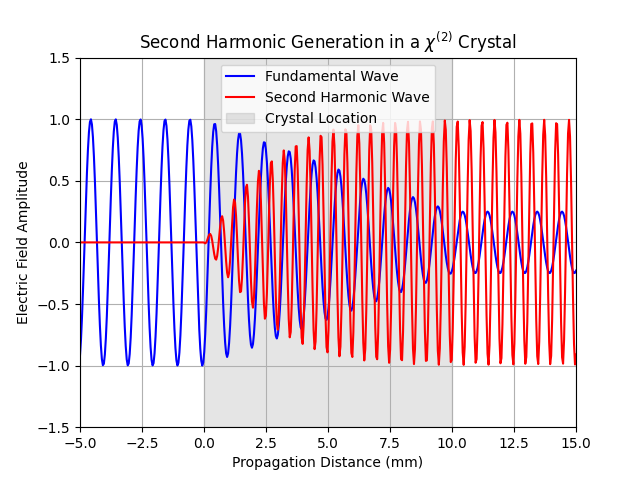
\includegraphics[width=0.8\textwidth]{../images/shg_snap.png}
    \caption{Snapshot from the animation showing the build-up of the second harmonic component during the propagation of the input pulse. Entire animation at: \href{https://i.giphy.com/media/v1.Y2lkPTc5MGI3NjExdm1nbWhlODkyeWljN21ydmRsa3prN3BhZWp2c29sbnl6b3g5NzQ0ayZlcD12MV9pbnRlcm5hbF9naWZfYnlfaWQmY3Q9Zw/bDFsLFIw86fGqPWW1a/giphy.gif}{Gify}}
    \label{fig:shg_visualization}
\end{figure}

The animation created from this simulation effectively demonstrates the key principles of second harmonic generation, providing a clear visual understanding of how the second harmonic wave emerges and evolves within the non-linear medium. This approach offers a valuable tool for visualizing and teaching the dynamic aspects of non-linear optical phenomena.

\subsection{Summary of Results}

The simulations presented in this section provide a comprehensive overview of the behavior of light in non-linear media under various conditions. The comparison between attosecond and CW lasers highlights the unique advantages of ultra-short pulse durations in driving non-linear effects. The Kerr effect and self-phase modulation were effectively demonstrated, along with the potential for quantum noise reduction through squeezing. High-order harmonic generation and cross-phase modulation were shown to be highly sensitive to the intensity and duration of the input pulses, while soliton interactions revealed complex dynamics that are crucial for applications in optical communication and other photonic technologies.

\newpage

\section{Conclusions}\label{sec:conclusion}

This study explored the simulation of various non-linear optical phenomena using Python, with a particular focus on attosecond lasers and their interactions with non-linear media. Through the simulations, we gained valuable insights into the behavior of light under extreme conditions and the potential applications of these phenomena in photonics.

Key conclusions drawn from the simulations include:

\begin{itemize}
    \item \textbf{Comparison of Attosecond and CW Lasers}: The comparison between attosecond and continuous wave (CW) lasers highlighted the unique capabilities of attosecond pulses in driving intense non-linear effects, such as spectral broadening and high-order harmonic generation, which are not as pronounced in CW lasers. This underscores the importance of pulse duration in non-linear optical applications.
    
    \item \textbf{Kerr Effect and Self-Phase Modulation (SPM)}: The simulation of the Kerr effect demonstrated how the intensity-dependent refractive index leads to self-phase modulation, resulting in significant spectral broadening. This phenomenon is critical for understanding the dynamics of ultra-short pulses in non-linear media and has implications for the design of advanced photonic devices.

    \item \textbf{Quantum Noise Reduction through Squeezing}: The simulations showed that non-linear interactions can effectively reduce quantum noise through squeezing, thereby enhancing the precision of quantum measurements. This finding is particularly relevant for applications in quantum optics and quantum information processing.

    \item \textbf{Second Harmonic Generation (SHG)}: The simulation and animation of the second harmonic generation process provided a clear visualization of how the second harmonic component emerges and evolves during pulse propagation. This visualization serves as an educational tool and offers insights into the conditions required for efficient harmonic generation.

    \item \textbf{Cross-Phase Modulation (XPM)}: The simulation of cross-phase modulation revealed the significant phase shifts and spectral changes induced by intense pulses interacting in a non-linear medium. These results are important for understanding and optimizing processes in optical communication and signal processing.

    \item \textbf{Optical Soliton Propagation}: The propagation simulation of optical solitons demonstrated their remarkable stability and shape preservation over long distances, even in the presence of small perturbations. This robustness makes solitons highly suitable for use in optical communication systems, where maintaining signal integrity is crucial.
    
\end{itemize}

Overall, this study has shown that Python is a powerful and versatile tool for simulating and understanding complex non-linear optical phenomena. The insights gained from these simulations not only enhance our understanding of fundamental physics but also pave the way for developing new technologies in photonics and quantum optics. Future research could build on this work by exploring more complex non-linear interactions, optimizing simulation techniques, and applying these findings to practical applications in communication, sensing, and quantum technologies.

\newpage

\section{Code Availability}

The Python code used for the simulations in this study is available on GitHub. The repository contains all scripts, and detailed instructions on how to reproduce the results presented in this paper.

The code can be accessed at the following link: \href{https://github.com/HeisenbergK/NLO}{GitHub}

I encourage the use of this code for further research and educational purposes. Any contributions, suggestions, or issues can be reported through the GitHub repository.

\nocite{*}
\bibliographystyle{ieeetr} % or any other style you prefer
\bibliography{bibliography}

\end{document}
